\def\circRad{4em}

\begin{figure}
    \centering
    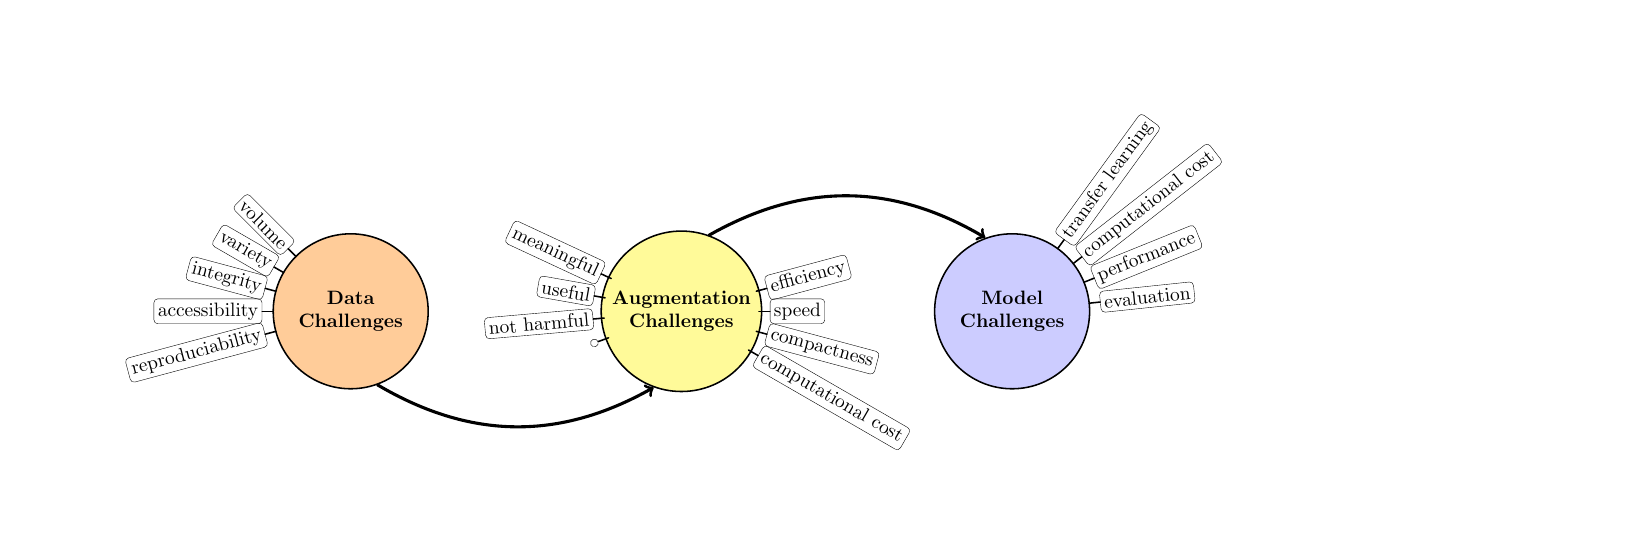
\begin{tikzpicture}[
    line cap=round, thick,
    stage/.style={shape=circle, draw, font=\bfseries, minimum width=2*\circRad},
    challenge/.style={draw, very thin, inner sep=2, rounded corners=2},
    every node/.style={align=center},
  ]
\centering
\scalebox{0.7}{
  \begin{scope}[local bounding box=challenges]
    % Data
    \node [stage, fill=orange!40] (data) {Data\\Challenges};
    \foreach \itm [count=\i, evaluate={\a=\i*15+120;}] in
      {volume, variety, integrity, accessibility, reproduciability} {
        \node[challenge] at (\a:\circRad + 2mm) [rotate=\a+180, anchor=east] {\itm};
        \draw (\a:\circRad + 2mm) -- (\a:\circRad);
      }

    % Transformations
    \begin{scope}[xshift=6cm]
      \node [stage, fill=yellow!40] (descriptor) {Augmentation\\Challenges};
      \foreach \itm [count=\i, evaluate={\a=\i*15+140;}] in
        {meaningful, useful, not harmful,} {
          \node[challenge] at (\a:\circRad + 2mm) [rotate=\a+180, anchor=east] {\itm};
          \draw (\a:\circRad + 2mm) -- (\a:\circRad);
        }
      \foreach \itm [count=\i, evaluate={\a=30-\i*15;}] in
        {efficiency, speed, compactness, computational cost} {
          \node[challenge] at (\a:\circRad + 2mm) [rotate=\a, anchor=west] {\itm};
          \draw (\a:\circRad + 2mm) -- (\a:\circRad);
        }
    \end{scope}

    % Model
    \begin{scope}[xshift=12cm]
      \node [stage, fill=blue!20] (model) {Model\\Challenges};
      \foreach \itm [count=\i, evaluate={\a=70-\i*16;}] in
        {transfer learning, computational cost, performance, evaluation} {
          \node[challenge] at (\a:\circRad + 2mm) [rotate=\a, anchor=west] {\itm};
          \draw (\a:\circRad + 2mm) -- (\a:\circRad);
        }
    \end{scope}
  \end{scope}

  \draw[ultra thick,->] (data.-70) to [bend right] (descriptor.-110);
  \draw[ultra thick,->] (descriptor.70) to [bend left] (model.110);
    }
\end{tikzpicture}
    \caption[Challenges in Data, Augmentation, and Model Stages]{\small{A visual representation of the challenges in three main stages of a machine learning pipeline: Data, Augmentation, and Model. The Data stage includes challenges such as volume, variety, integrity, accessibility, and reproducibility. The Augmentation stage covers challenges related to creating meaningful, useful, and not harmful augmentations while considering efficiency, speed, compactness, and computational cost. The Model stage addresses challenges in transfer learning, computational cost, performance, and evaluation. Arrows indicate the flow of progression from one stage to another.}}

    \label{fig:my_label}
\end{figure}